\section{Numerical validation}
\label{sec:numerics}

The experiments follow the main theory: first verify full-ridge risk and derivatives, then optimal weights and gains, followed by surrogate dosage, first-order exchange, and the limits of nonlinear learners and real visual features. All evidence is controlled-model evidence, not external validation of robot policies.

\paragraph{Protocol.}
Unless stated otherwise, synthetic experiments use Gaussian covariates, a shared spectral basis, $\sigma_r^2=1$, $\sigma_h^2=4$, $\mu=0.05$, and $\nr=1000,\nh=6000$. E1 is diagonalized ridge, E2 is standard full ridge, E3 is a linear model trained by full-batch Adam with explicit $L_2$, and E4 is a small MLP. Design-level conditional risks are distinguished from actual-E2 fits, oracle grid minima, and validation-selected decisions.

\subsection{Full-ridge risk and derivative checks}
\label{sec:numerics-risk}

The fixed-dimension second-order risk expansion is checked in 22 design-level cells over $p=1,2,20$, aligned and anti-aligned mismatch, and $\lambda=0,0.1,0.3,0.5,0.8,1$. All simulated means are within $2.13$ Monte-Carlo standard errors of the prediction; three direct actual-estimator checks are within $1.12$ standard errors. Compact matrix coefficients, independent pairwise expansion, and zero-mixing consistency have maximum discrepancy $7.11\times10^{-15}$.
For the zero-mixing derivative, six cells give agreement within sampling and higher-order error: for spectral family A at $p=20$, $\nr=1000$ gives prediction $0.0148136$ and Monte Carlo $0.0147617\pm0.0000197$, while $\nr=16000$ gives $0.0263331$ and $0.0263323\pm0.0000052$. Direct actual-estimator finite differences at $\lambda=10^{-4}$ give $0.0143334\pm0.0003422$ for the former cell. These checks support the full-ridge risk and derivative objects, not an exact finite-sample root.

\subsection{Optimal weight and optimized-gain checks}
\label{sec:numerics-optimum}

For a two-dimensional aligned example with a unique interior optimum, the population minimizer is $w_0=0.3708597$ with $R_0''(w_0)=0.13996$. The predicted optimized risks at $\nr=1000,4000$ are $0.01063196$ and $0.01002290$, compared with Monte Carlo $0.01063452$ and $0.01002470$. Four optimized-risk checks are within $1.59$ standard errors, supporting the interior nondegenerate theorem.
The same example has $R_1'(w_0)=0.320971$ and predicted scaled weight shift $-R_1'(w_0)/R_0''(w_0)=-2.29329$. At $\nr=4000$, 200{,}000 conditional-design replicates give $-2.29688\pm0.07803$ for $\nr(w_n^*-w_0)$. Independent actual-E2 paired checks at $\nr=1000$ give negative and positive derivatives on the two sides of the first-order weight prediction, respectively $-0.000435\pm0.000137$ and $0.000469\pm0.000137$.
The local--global counterexample is also reproduced: at $\nr=1000$, its zero-mixing derivative is $0.2265$, yet its optimal gain is $0.00936$; independent actual-E2 paired gain is $0.009266\pm0.000372$. This confirms that the local derivative cannot replace a global optimum calculation.

Two pre-registered direct-$n_r$ tests further pass the 20\% root-compatibility criterion. The p2 anti-aligned predicted root is $55.644$, estimated root $61.750$, with Bonferroni 97.5\% root-ratio interval $[1.082,1.137]$; p20 spectral A gives $453.395$, $464.610$, and $[1.008,1.041]$. Actual-E2 paired differences have the same sign on both sides of each root. These are boundary checks, not a substitute for the optimal-weight checks above.

\begin{figure}[t]
  \centering
  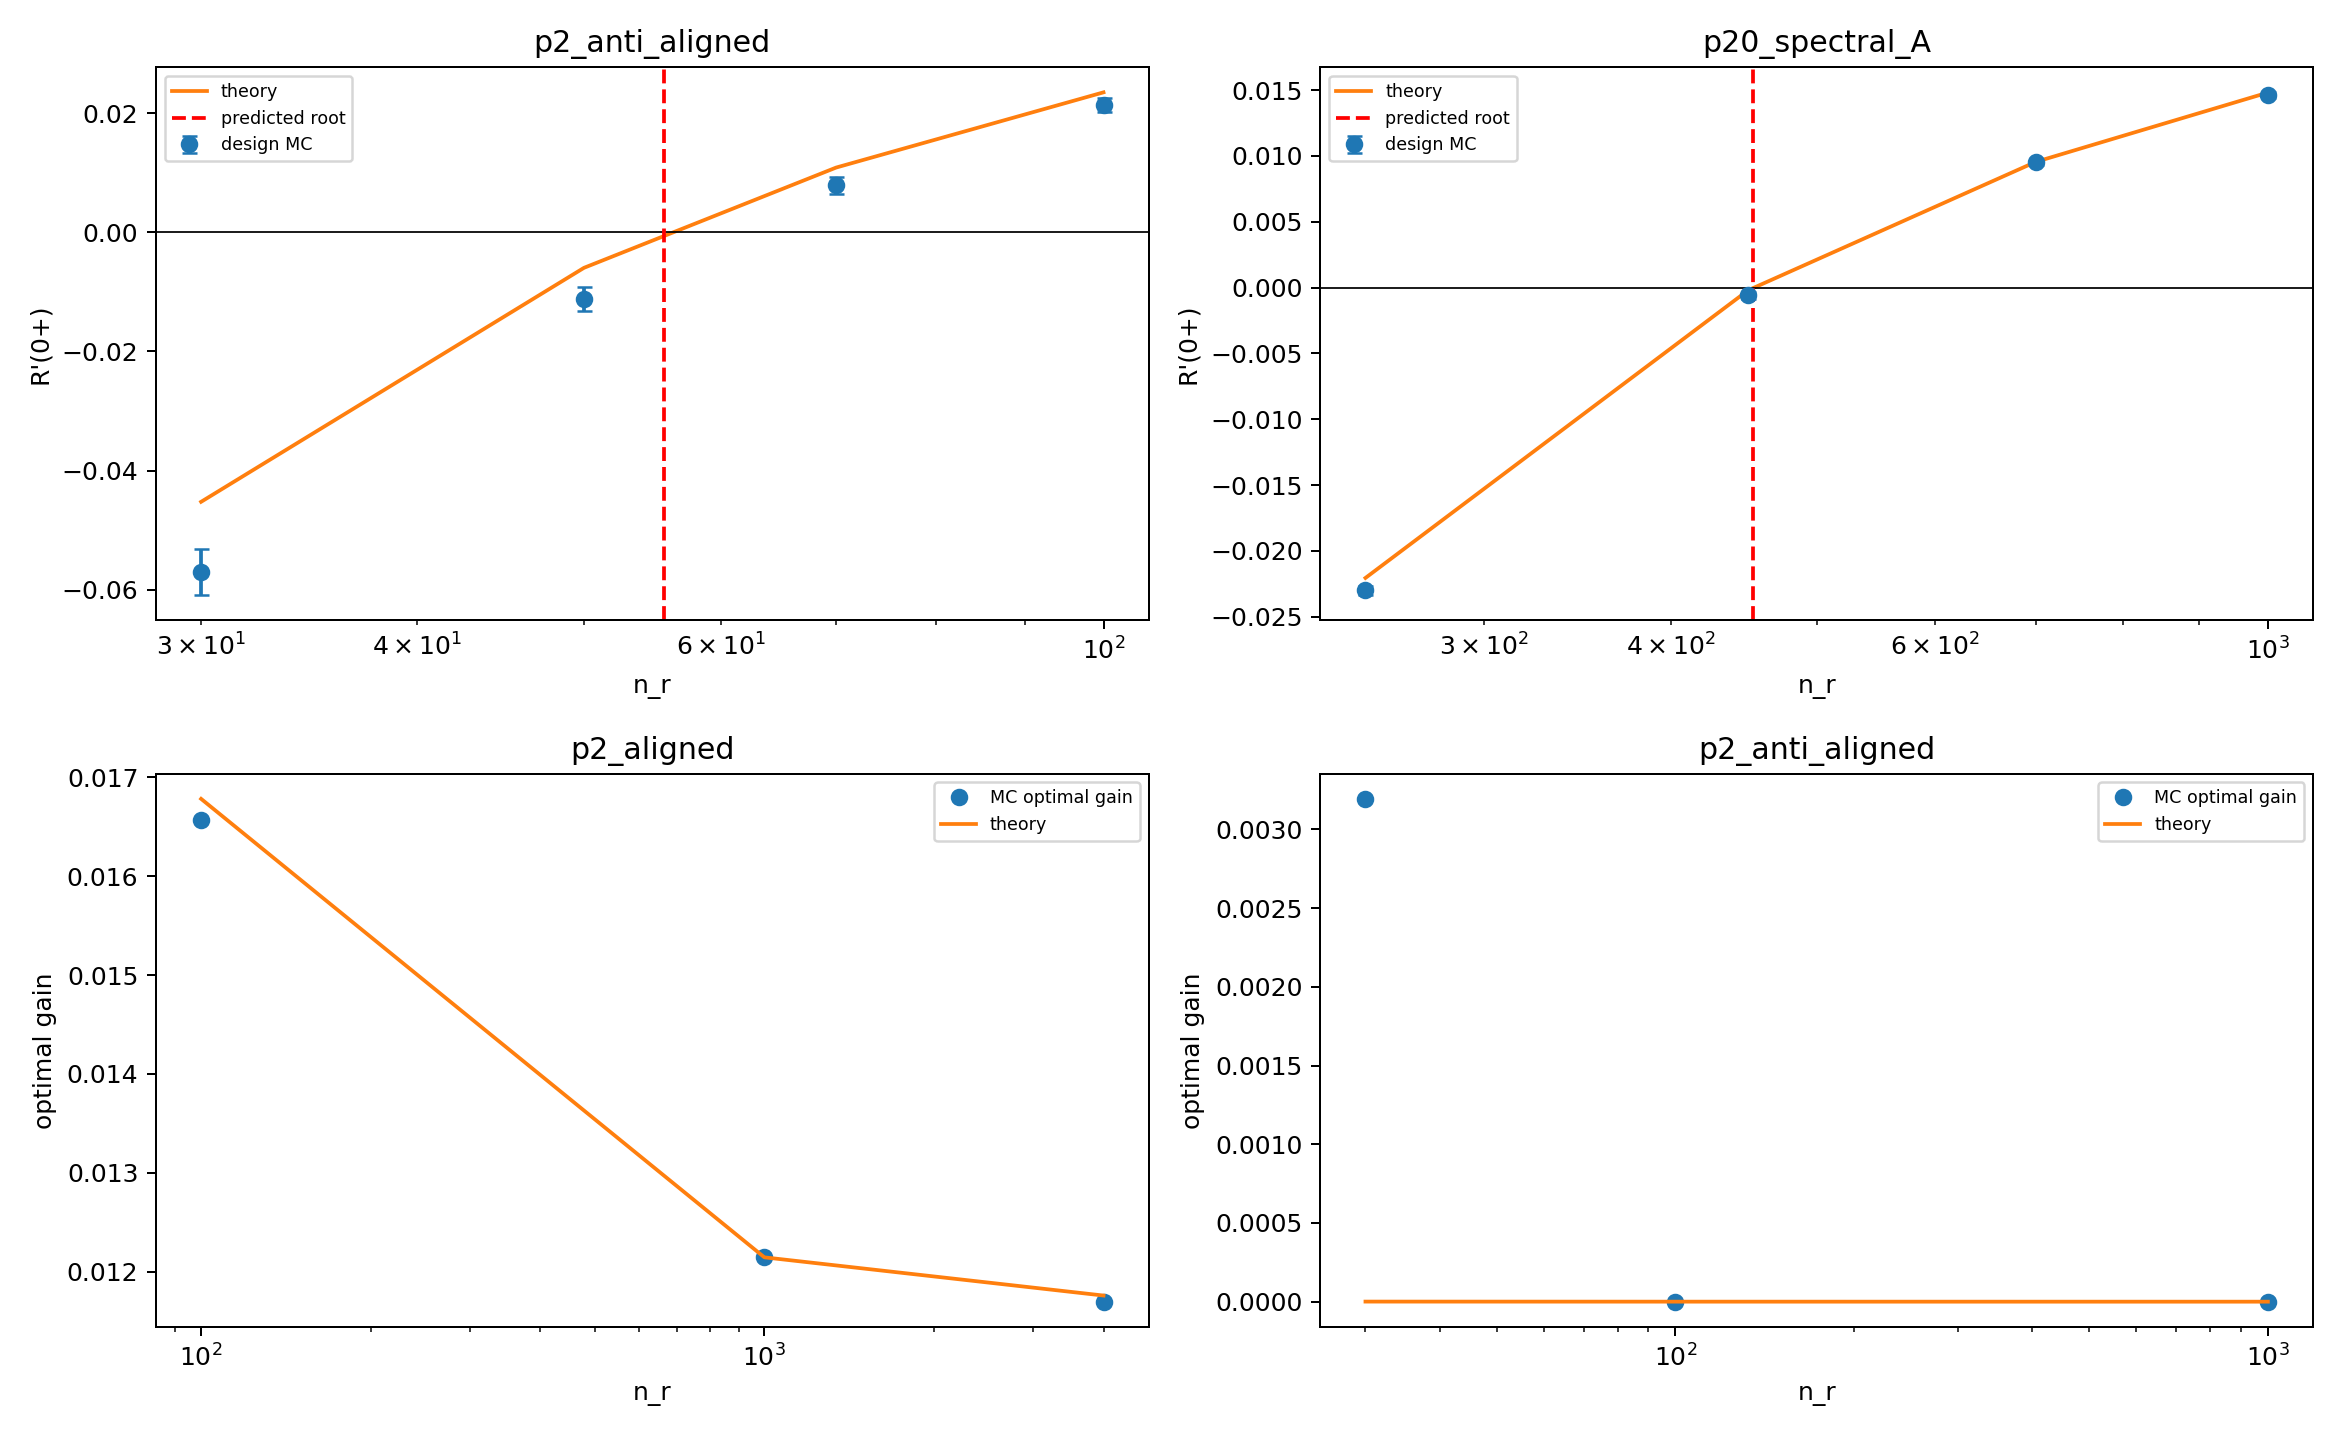
\includegraphics[width=\linewidth]{fig/s5_overview.png}
  \caption{\textbf{Full-ridge risk, boundary, and optimized-gain checks.} Top: design-level zero-mixing derivatives and theory across $n_r$, with predicted roots marked. Bottom: optimal gains for representative configurations. Raw JSON and the preregistration are provided in the supplementary repository.}
  \label{fig:s5overview}
\end{figure}

\subsection{Surrogate dosage and first-order exchange}
\label{sec:numerics-dosage}

Across 16 configurations, the closed-form surrogate optimum agrees with grid minimization of the same surrogate to within $1.49\times10^{-10}$ in gain. The checks cover its interior and boundary branches, including a surrogate crossing to $w=1$ at $\nh=1779.17$; they test the algebraic implementation. A separate full-ridge conditional-risk experiment evaluates the optimized-gain expansion, giving $0.0122262\pm0.0000066$ versus prediction $0.0122186$ in one configuration. Exchange checks evaluate the first-order equation: no-finite-solution cells at $\nr=1000$ and a finite algebraic example $\kex^{(1)}=2.8527963$ at $\nr=40,\rho=6$.

\begin{figure}[t]
  \centering
  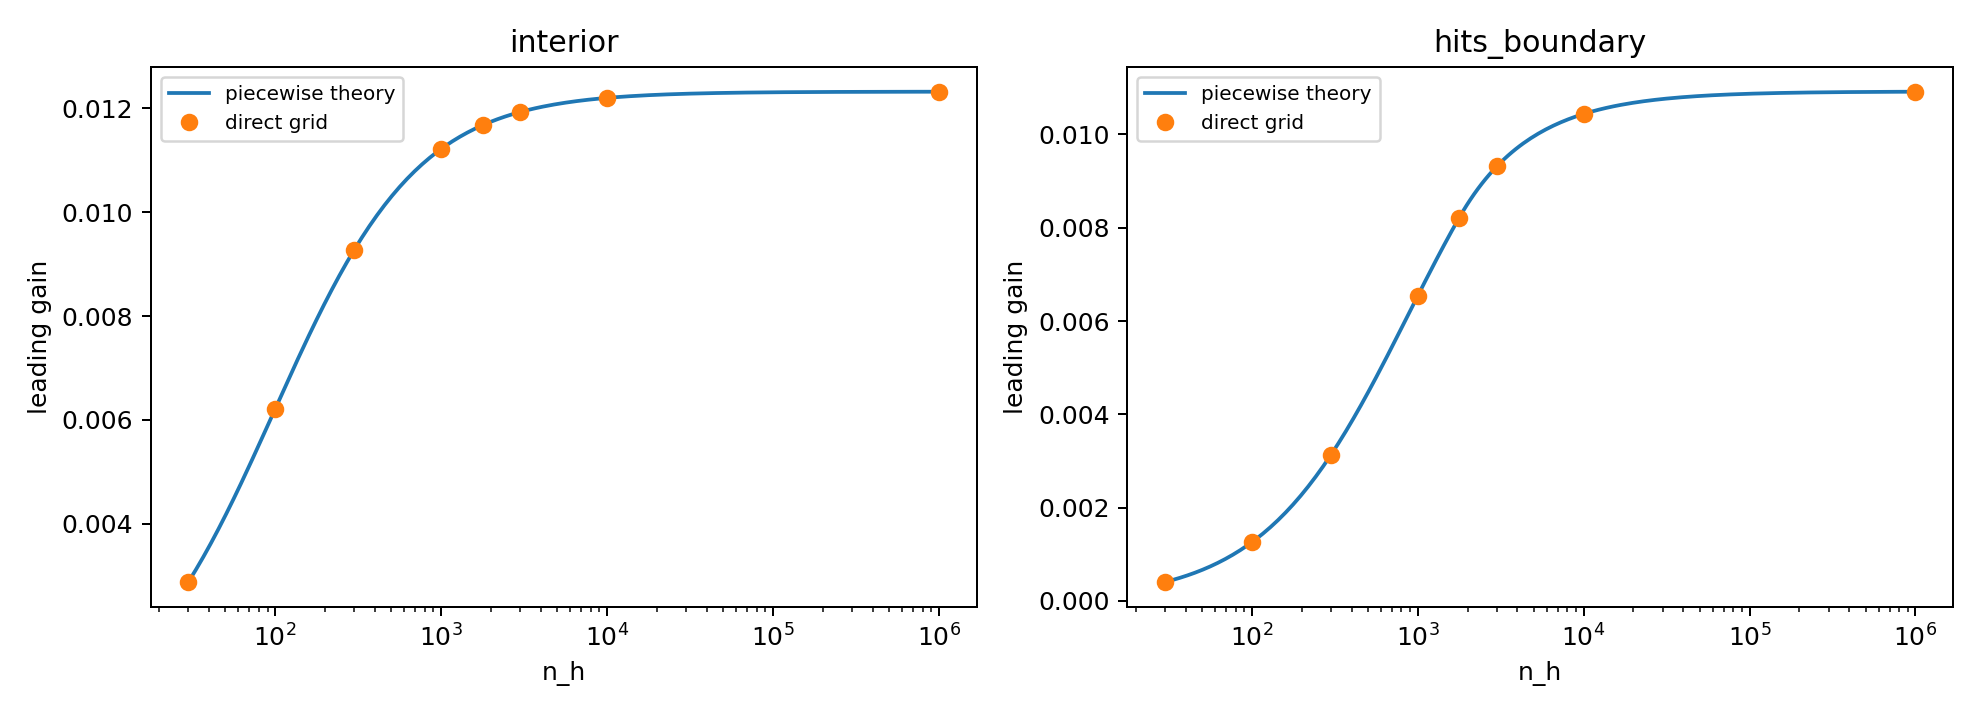
\includegraphics[width=\linewidth]{fig/s5_dosage.png}
  \caption{\textbf{Piecewise dosage rule for the quadratic surrogate.} Curves show its exact interior and $w=1$ boundary solutions; points are grid minima of the same surrogate. This is an algebraic consistency check, not a full-ridge risk experiment.}
  \label{fig:s5dose}
\end{figure}

\subsection{Nonlinear learners and real visual features}
\label{sec:numerics-real}

The small-MLP arm exhibits mixing benefits, but the optimum and risk magnitude are learner-dependent. For example, MLP and full-ridge optimal weights are respectively $0.05$ versus $0.40$ for p2 aligned, $0.40$ versus $0.70$ for p2 anti-aligned at $\nr=50$, and $0.10$ versus $0.00$ at $\nr=70$. Thus, the mechanism can persist beyond ridge while the optimal weight and regularization change. The small-MLP results are not quantitative equivalence validation.
E3 full-batch Adam reproduces the full-ridge curve to machine precision (median relative error $10^{-15}$), an optimizer--objective identity check. The earlier single-seed E4 arm deviates materially (median $\sim32\%$) and remains exploratory.

\begin{figure}[t]
  \centering
  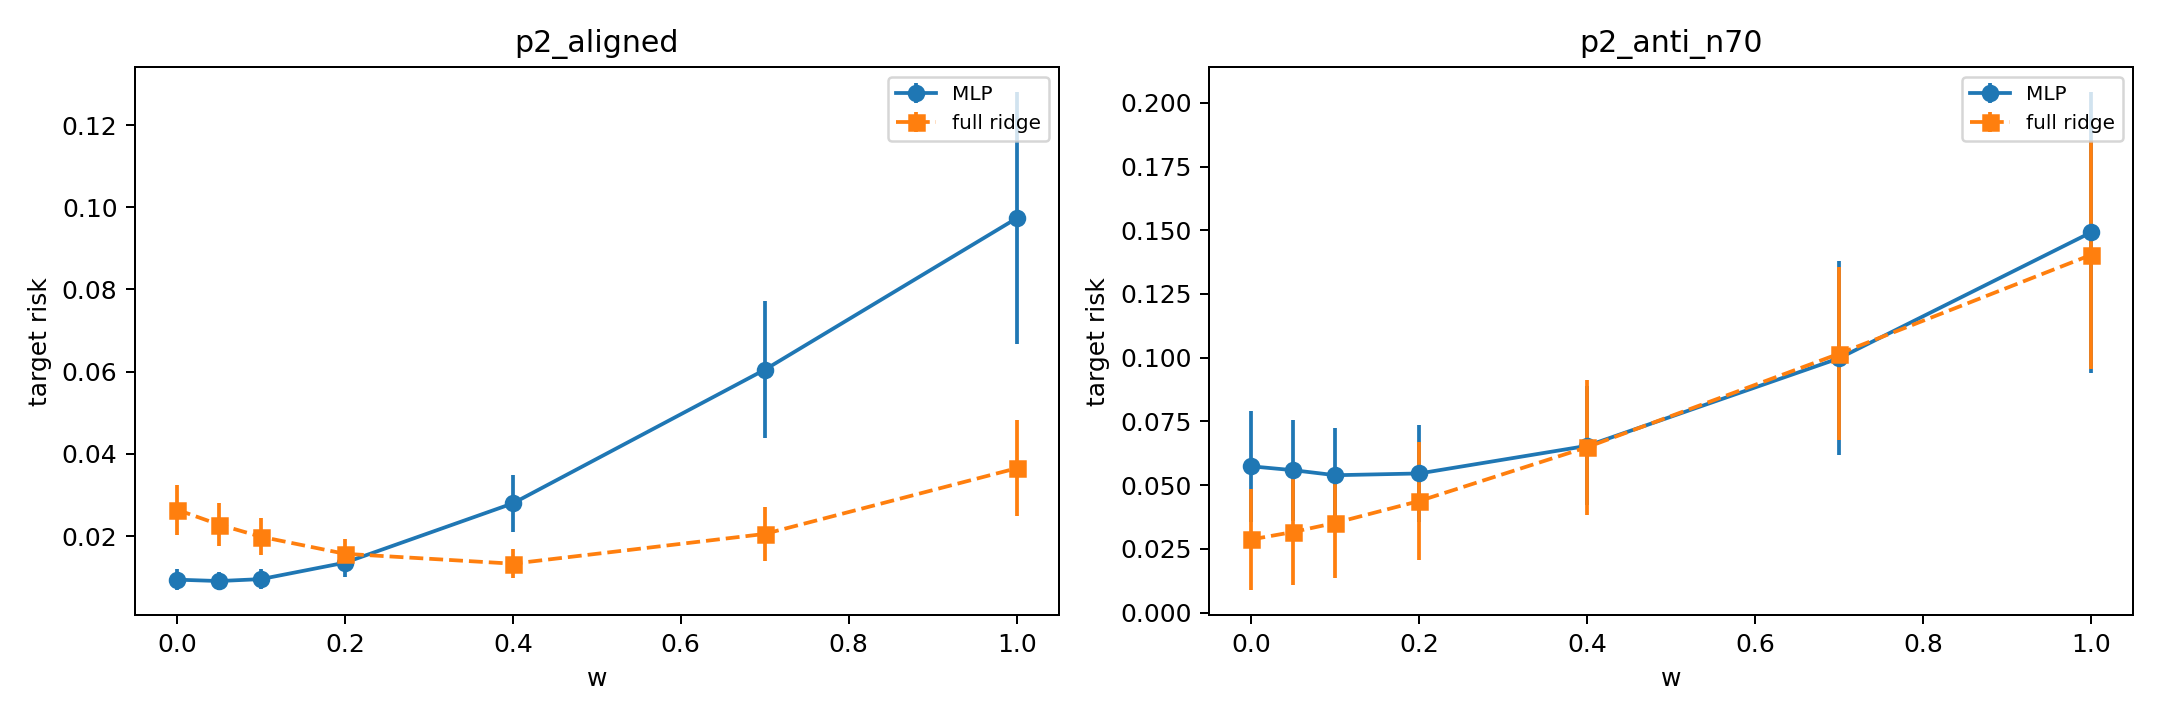
\includegraphics[width=\linewidth]{fig/nonlinear_risk_curves.png}
  \caption{\textbf{Learner-dependent risk curves.} Small MLP and full ridge can both benefit from mixing, but their optimal weights and risk magnitudes differ. Five seeds are used with baseline L2 calibration.}
  \label{fig:nonlinear}
\end{figure}

The real-feature arm uses frozen grayscale PCA fitted only on training data and controlled regression labels, not CIFAR class labels. Both $w$ and $\mu$ are selected using only noisy target validation labels, with $\mu$ tuned separately for each $w$. The resulting gains are strongly mismatch dependent and are not uniformly positive: for low-frequency mismatch, the gains at $\nr=50,200,2000$ are $0.00260$, $-0.00739$, and $-0.00076$; for white mismatch they are $0.16193$, $0.02461$, and $-0.00016$; for high-frequency mismatch they are $0.30420$, $0.06313$, and $0.00156$. Thus, ordinary validation does not always realize the oracle mixing gain, especially for low-frequency mismatch, while the high-frequency gains remain positive but decrease with target sample size. Selected weights generally decrease as target data grow, and fixed $w=0.5$ can be strongly harmful for low-frequency mismatch. These results support sample-size- and mismatch-dependent mixing on real visual features, not a universal mixture rule, a guaranteed validation-selected gain, or a real robot task.

\begin{figure}[t]
  \centering
  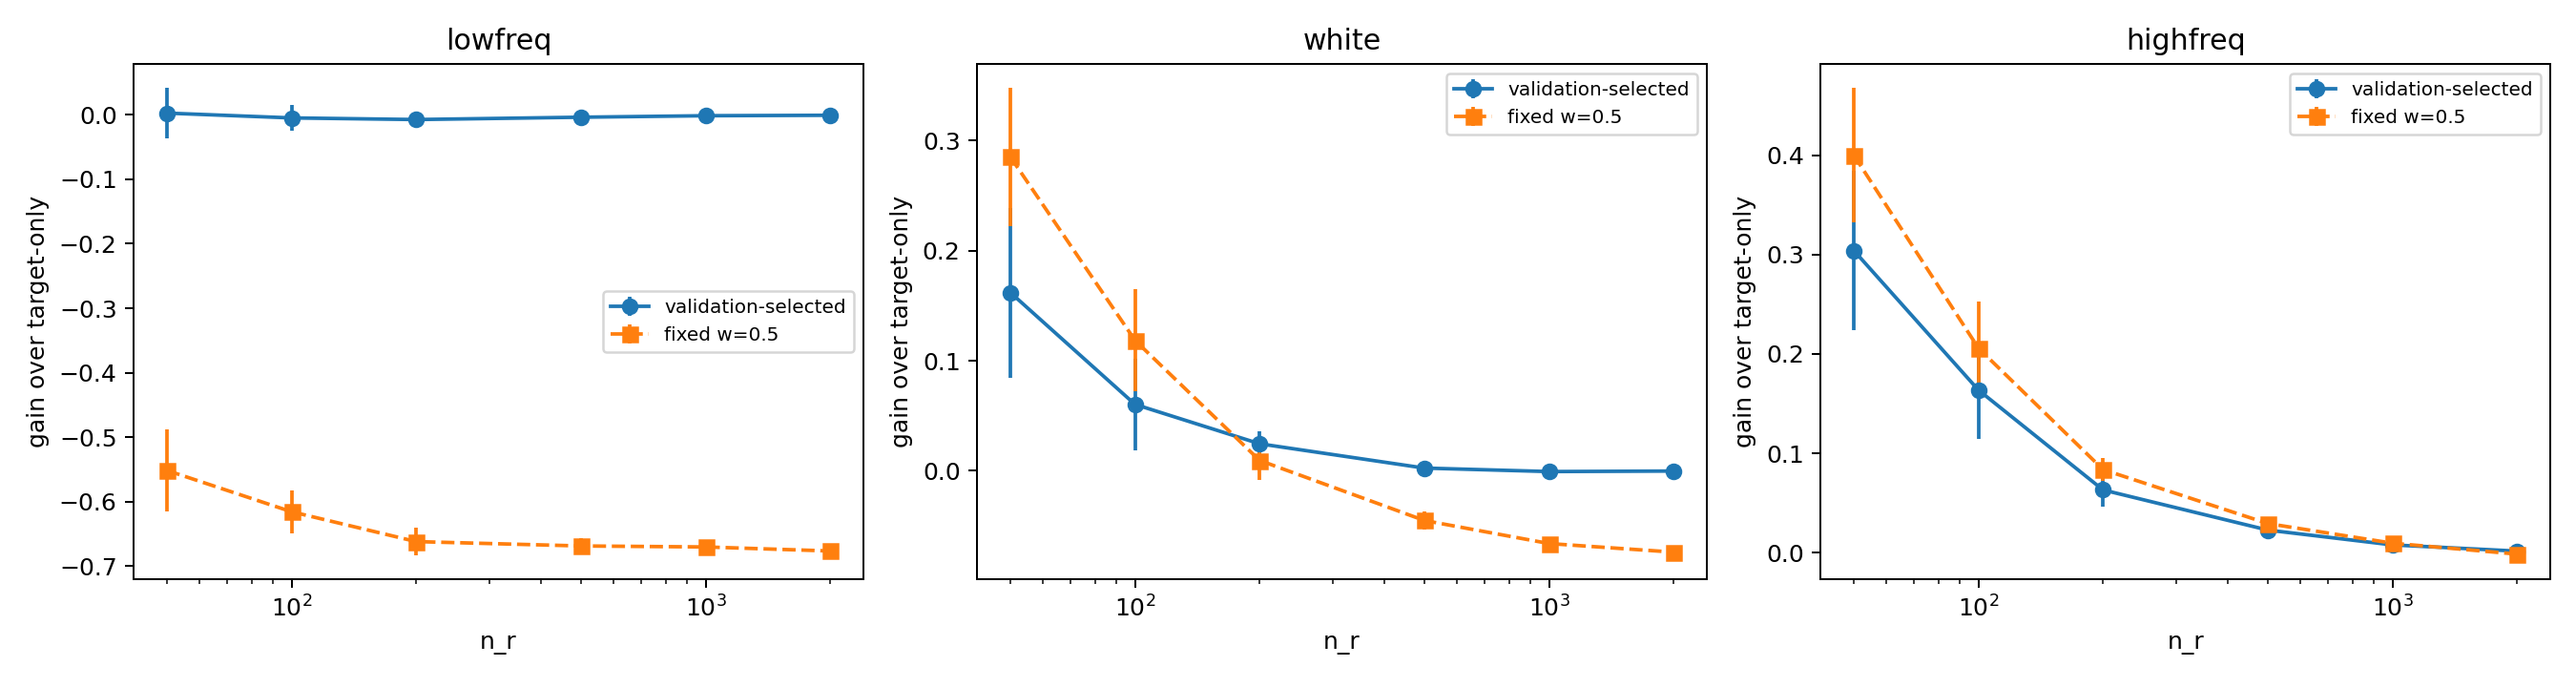
\includegraphics[width=\linewidth]{fig/cifar_gain_curves.png}
  \caption{\textbf{Real-feature mixing gains.} Validation-selected and fixed $w=0.5$ gains under three mismatch shapes. Selection uses noisy validation labels only, with $\mu$ tuned separately for each $w$; test data and $\beta^*$ do not enter selection. Error bars are 95\% normal-confidence intervals across replicates. The controlled labels are synthetic regression labels, not the original CIFAR classes.}
  \label{fig:cifar}
\end{figure}

\subsection{Special cases and robustness checks}
\label{sec:numerics-robustness}

The diagonalized E1 formula matches Monte Carlo to a median relative error of $0.15\%$. Its independent dosage check gives $\chi^2=11.124$, df $=11$, $p=0.433$, with fitted half-saturation $3541$ (bootstrap 95\% CI $[2948,4243]$) versus $3624$ theoretically; this is within-model compatibility, not equivalence validation. The older E2 strict $1/g$-linearity gate fails ($R^2=0.92571$), so that precise dosage form is not established beyond E1.
The E1 low-frequency root estimate is $0.3756$ with 95\% CI $[0.3286,0.4288]$, containing the finite-$\nr$ theoretical root $0.3821$; older E2/E3 point-boundary gates fail. Basis-rotation errors grow from $0.96\%$ to $30.5\%$ for E2, but the rotation also changes task mismatch, so it is not a clean basis-only causal test. Mismatch-location contrasts additionally vary target-weighted energy and alignment, and are not independent location theorems. These results delimit the model and should not be read as general robustness claims.
